\chapter{Análisis de Fourier y características espectrales}
\label{cap:fourier}

\section{Serie y transformada de Fourier}

Una señal periódica de período $T$ y energía finita en un período admite la representación
\begin{equation}
x(t) = \sum_{k=-\infty}^{\infty} c_k\, e^{i 2\pi k t / T},\qquad c_k = \frac1T\int_0^T x(t)\,e^{-i2\pi k t/T}\,dt.
\end{equation}
Para señales no periódicas de energía finita se define la transformada de Fourier
\begin{equation}
X(f) = \int_{-\infty}^{\infty} x(t)\, e^{-i 2\pi f t}\, dt, \qquad x(t) = \int_{-\infty}^{\infty} X(f)\, e^{i 2\pi f t}\, df.
\end{equation}

\pendiente{propiedades: linealidad, desplazamiento, convolución $\leftrightarrow$ producto (base del filtrado); referencia a \cite{gonzalez2018}, cap.~4, y \cite{oppenheim2010}.}

\section{Muestreo y transformada discreta}

\paragraph{Teorema de muestreo (Nyquist--Shannon).} Si $X(f) = 0$ para $|f| > f_{\max}$, la señal queda completamente determinada por sus muestras $x[n] = x(n/f_s)$ siempre que $f_s > 2 f_{\max}$. Con $f_s = 256$~Hz la frecuencia de Nyquist es 128~Hz, muy por encima de los 45~Hz que se analizan.

\paragraph{Transformada discreta de Fourier (DFT).} Para $x[n]$, $n=0,\dots,N-1$:
\begin{equation}
X[k] = \sum_{n=0}^{N-1} x[n]\, e^{-i 2\pi k n/N}, \qquad f_k = \frac{k f_s}{N},\quad k = 0,\dots,N-1.
\label{eq:dft}
\end{equation}
La FFT la calcula en $O(N\log N)$ operaciones en lugar de $O(N^2)$.

\begin{teorema}[Parseval, versión discreta]\label{teo:parseval}
\[
\sum_{n=0}^{N-1} |x[n]|^2 = \frac1N \sum_{k=0}^{N-1} |X[k]|^2.
\]
\end{teorema}
\begin{proof}
Sea $\omega = e^{-i2\pi/N}$. Entonces
\[
\sum_k |X[k]|^2 = \sum_k \sum_n \sum_m x[n]\,\overline{x[m]}\,\omega^{k(n-m)}
= \sum_n \sum_m x[n]\,\overline{x[m]} \sum_k \omega^{k(n-m)}.
\]
La suma geométrica $\sum_{k=0}^{N-1}\omega^{k(n-m)}$ vale $N$ si $n=m$ y $0$ en otro caso (porque $\omega^{N(n-m)}=1$ y $\omega^{n-m}\neq 1$). Queda $\sum_k|X[k]|^2 = N\sum_n |x[n]|^2$.
\end{proof}

El teorema justifica interpretar $|X[k]|^2$ como la distribución de la energía de la señal entre las frecuencias $f_k$. En el notebook (sección~3) se verifica numéricamente sobre una ventana de EEG, con una diferencia relativa del orden de $10^{-16}$.

\section{Estimación de la densidad espectral de potencia}

\subsection{Periodograma y fuga espectral}

Cortar la señal a una ventana finita equivale a multiplicarla por una función rectangular; en frecuencia, eso es convolucionar con un núcleo de tipo $\operatorname{sinc}$ cuyos lóbulos laterales ``derraman'' potencia hacia frecuencias vecinas (\emph{fuga espectral}). Usar una ventana de Hann, $w[n] = \tfrac12\big(1 - \cos\tfrac{2\pi n}{N}\big)$, reduce fuertemente los lóbulos laterales a cambio de ensanchar el lóbulo principal.

\subsection{Método de Welch}

El periodograma de una sola ventana es un estimador \emph{inconsistente}: su varianza no disminuye al aumentar $N$. \textcite{welch1967} propuso dividir la señal en $K$ segmentos solapados de longitud $L$, ventanear cada uno y promediar:
\begin{equation}
\hat P(f_k) = \frac{1}{K}\sum_{j=1}^{K} \frac{1}{f_s \sum_n w[n]^2}\Big|\sum_{n=0}^{L-1} w[n]\, x_j[n]\, e^{-i2\pi kn/L}\Big|^2.
\label{eq:welch}
\end{equation}
Si los segmentos fueran independientes, la varianza se reduciría en un factor $K$. En este trabajo cada ventana de 4~s se divide en segmentos de 1~s con 50~\% de solapamiento ($K=7$), lo que da una resolución de 1~Hz.

\pendiente{figura \texttt{fourier\_normal\_vs\_crisis} y su discusión.}

\begin{figure}[ht]
\centering
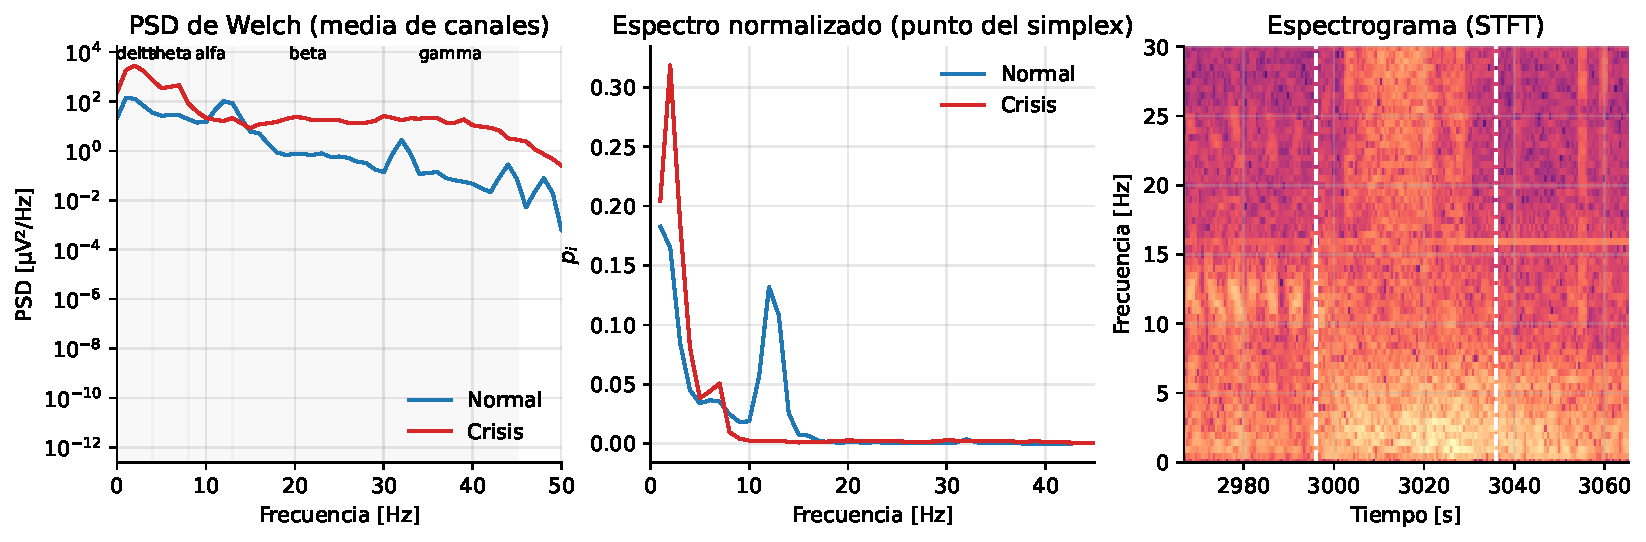
\includegraphics[width=\linewidth]{fourier_normal_vs_crisis}
\caption{Izquierda: PSD de Welch de una ventana normal y una de crisis. Centro: el mismo espectro normalizado, que es un punto del simplex. Derecha: espectrograma alrededor de la crisis.}
\label{fig:fourier}
\end{figure}

\section{Características espectrales}

Para cada canal y cada ventana se calculan:
\begin{itemize}
  \item \textbf{Potencia por banda:} $P_b = \sum_{f_k \in b} \hat P(f_k)$, en escala logarítmica.
  \item \textbf{Potencia relativa:} $r_b = P_b / \sum_{b'} P_{b'}$.
  \item \textbf{Entropía espectral} (sección~\ref{sec:entropia}).
  \item \textbf{Frecuencia dominante} $\arg\max_k \hat P(f_k)$ y \textbf{frecuencia de borde espectral} al 90~\%.
  \item \textbf{Line length} $\frac1N\sum_n |x[n+1]-x[n]|$ y log-varianza, como referencia en el dominio del tiempo.
\end{itemize}

\subsection{Coherencia entre canales}

La coherencia de magnitud cuadrada entre los canales $a$ y $b$ es
\begin{equation}
C_{ab}(f) = \frac{|S_{ab}(f)|^2}{S_{aa}(f)\,S_{bb}(f)} \in [0,1],
\end{equation}
donde $S_{ab}$ es la densidad espectral cruzada estimada también con Welch. Por la desigualdad de Cauchy--Schwarz, $|S_{ab}|^2 \le S_{aa}S_{bb}$, y vale 1 si y solo si los dos canales están relacionados por un sistema lineal. Es la medida espectral natural de la sincronización que caracteriza a una crisis.

\section{Entropía espectral, el simplex y multiplicadores de Lagrange}
\label{sec:entropia}

Al normalizar la PSD en las $N$ frecuencias de interés, $p_i = \hat P(f_i)/\sum_j \hat P(f_j)$, se obtiene un vector del \emph{simplex de probabilidad}
\begin{equation}
\simplex = \Big\{ p\in\R^N : p_i \ge 0,\ \sum_{i=1}^N p_i = 1\Big\}.
\end{equation}
El simplex es convexo y compacto: es la envolvente convexa de los $N$ vectores canónicos $e_1,\dots,e_N$. Un vértice $e_i$ representa una señal con toda su potencia en una sola frecuencia, y el baricentro $(1/N,\dots,1/N)$ representa ruido blanco.

\begin{definicion}
La \emph{entropía espectral} es $H(p) = -\sum_{i=1}^N p_i \log p_i$ (con $0\log 0 = 0$) \parencite{inouye1991}.
\end{definicion}

\begin{proposicion}\label{prop:max_entropia}
$\max_{p\in\simplex} H(p) = \log N$, y el máximo se alcanza únicamente en $p^\star = (1/N,\dots,1/N)$.
\end{proposicion}
\begin{proof}
\emph{Punto crítico.} Se plantea el lagrangiano con la restricción de igualdad:
\[
\mathcal{L}(p,\lambda) = -\sum_i p_i\log p_i + \lambda\Big(\sum_i p_i - 1\Big).
\]
La condición de primer orden $\partial\mathcal{L}/\partial p_i = -\log p_i - 1 + \lambda = 0$ da $p_i = e^{\lambda-1}$, el mismo valor para todo $i$. Con la restricción $\sum_i p_i = 1$ resulta $p_i = 1/N$ y $\lambda^\star = 1 - \log N$. En ese punto $H(p^\star) = \log N$.

\emph{Restricciones de desigualdad.} En $p^\star$ todas las componentes son positivas, así que las restricciones $p_i\ge 0$ no están activas y sus multiplicadores de KKT son nulos. Además, $\partial H/\partial p_i \to +\infty$ cuando $p_i \to 0^+$, de modo que ningún máximo puede estar en el borde del simplex.

\emph{Globalidad y unicidad.} El Hessiano es $\nabla^2 H(p) = -\operatorname{diag}(1/p_1,\dots,1/p_N) \prec 0$ en el interior del simplex: $H$ es estrictamente cóncava sobre un conjunto convexo. En un problema de maximización cóncava todo máximo local es global, y la concavidad estricta garantiza que es único.
\end{proof}

Se usa la entropía normalizada $\tilde H = H/\log N\in[0,1]$. Por la proposición~\ref{prop:max_entropia}, $\tilde H = 1$ corresponde a una potencia repartida uniformemente y $\tilde H \to 0$ a una potencia concentrada en una sola frecuencia. Según el modelo del capítulo~\ref{cap:senal}, una crisis desplaza $p$ hacia un vértice del simplex, lo que motiva la hipótesis~\ref{h:entropia}.

En el notebook (sección~4) se resuelve numéricamente el problema con un método de región de confianza con restricciones, desde varios puntos iniciales: siempre converge a $p^\star$ y al multiplicador $\lambda^\star = 1-\log N$.

\begin{figure}[ht]
\centering
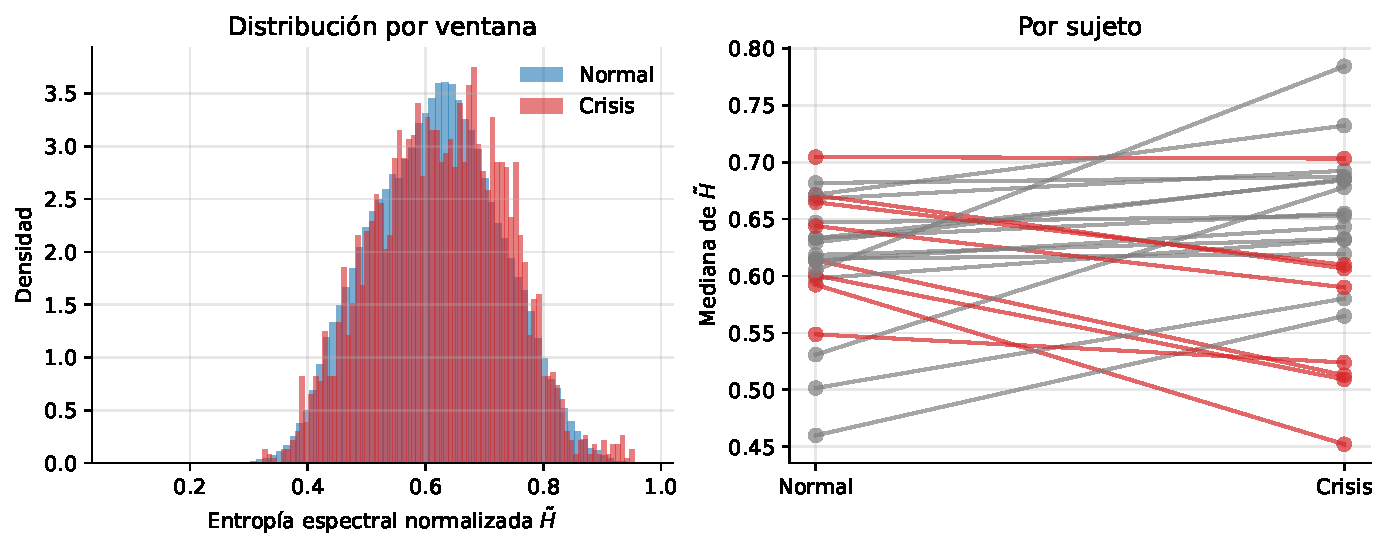
\includegraphics[width=\linewidth]{h5_entropia}
\caption{Entropía espectral normalizada en ventanas normales y de crisis (izquierda) y mediana por sujeto (derecha).}
\label{fig:h5}
\end{figure}

\pendiente{resultados numéricos de H5 (salida de la sección 5 del notebook).}
